\section{A API DSL cotas}
\label{apicotas}

Em relação ao desafio abordado nos objetivos específicos dessa pesquisa, no que diz respeito à evolução entre as versões e à geração de código fonte de classificação e aprovação de candidatos, foi criada uma \gls{API} para prova de conceito sobre o uso dos padrões das regras definidas na DSL Cotas. Esta por sua vez implementa os algoritmos responsáveis por calcular o quadro de vagas, aprovar candidatos e definir a ordem de prioridade conforme as regras definidas pelo usuário.


Para tanto, a tecnologia escolhida foi o projeto \texttt{SpringBoot}, o qual segundo \citeonline{walls2016spring}, oferece um novo paradigma de desenvolvimento de aplicações com o \texttt{Spring Framework}, possibilitando desenvolver aplicativos com mais agilidade, focando em atender as necessidades de funcionalidade com o mínimo de configurações que for necessário.

No que concerne à escolha para criação de serviços web, o setor de desenvolvimento do \gls{IFSC} possui dois sistemas que envolvem processos seletivos, o primeiro é o sistema legado em \texttt{PHP}, tratado no Capítulo \ref{chap:historicoversoes} e o segundo é o novo Sistema Integrado de Gestão (SIG) que também contém um módulo responsável pela criação de processos seletivos e foi desenvolvido em \texttt{Java}. Portanto, a camada de serviços foi empregada com o intuito de permitir a utilização em sistemas distintos de modo independente de linguagem alvo para geração de código fonte.


Nas próximas Subseções são detalhados os recursos do \texttt{Spring} que foram utilizados na criação das funcionalidades de classificação e aprovação de candidatos.


\subsection{Componentes da API}
\label{componentesapi}

Inicialmente, foi gerado um projeto \texttt{SpringBoot} por meio do site \texttt{start.spring.io}, no qual foram marcadas as opções de módulos necessários para o desenvolvimento da pesquisa, tais como:

\begin{enumerate}
 
\item[a)] \texttt{Spring Boot Starter Web}: Principal dependência do \texttt{Spring}, que fornece a camada de desenvolvimento utilizada para construção de aplicações e serviços web com o \texttt{spring-web}, incluindo um \texttt{tomcat} pré configurado e a biblioteca \texttt{jackson}, para fazer manipulação de (JSON ou XML);


\item[b)] \texttt{Spring Data JPA}:  Utilizado para simplificar a criação, seleção e manipulação das entidades de banco de dados criadas para processar o algoritmo de classificação e aprovação de candidatos; 

\item[c)] \texttt{JDBC API}: Para fornecer acesso ao banco de dados \texttt{MYSQL} do sistema de ingresso, utilizado para validação e possibilitar a comparação de resultados do histórico de candidatos dos processos do \gls{IFSC} com o resultado processado pela \gls{API} DSL Cotas; 


\item[d)] \texttt{Spring Reactive Web}: Módulo do \texttt{Spring} utilizado para testar as requisições para os \texttt{endpoints} implementados com base na DSL, por meio do \texttt{WebClient} em conjunto com o \texttt{JUnit}.

\end{enumerate}



Após a inicialização do projeto foram criadas as entidades de modelo necessárias para fazer o mapeamento do arquivo JSON gerado pela DSL Cotas, para isso, foram utilizadas as anotações \texttt{Json}, disponíveis pela biblioteca \texttt{jackson}. Um exemplo do mapeamento é apresentado pela Figura \ref{fig:jsonjackson}. 

\begin{figure}[ht!]
\centering

\caption{\textmd{Anotações com a biblioteca jackson}}
\label{fig:jsonjackson}
\fcolorbox{gray}{white}{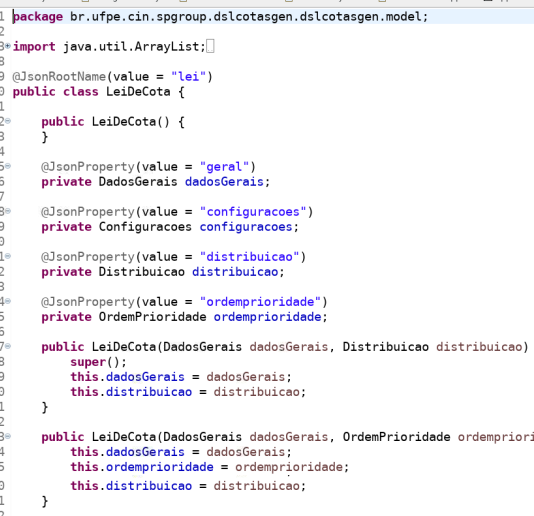
\includegraphics[width=0.80\textwidth]{chapters/dslcotas/api/imagens/jsonjackson.png}}

\par\medskip\textbf{Fonte:} Elaboração do autor (2020) \par\medskip

\end{figure}



Desse modo, o modelo de regras gerado pela DSL Cotas é convertido para o objeto instância da classe \texttt{LeiDeCota}, que possui toda a estrutura de dados utilizada para armazenar e percorrer as regras definidas pelo usuário.

A API possui um controlador \texttt{REST} para cálculo de cotas, o qual fornece acesso às requisições \texttt{HTTP} que têm a função de: gerar o quadro de vagas, retornar a ordem de prioridade e aprovar uma lista de candidatos. Esse controlador por sua vez, utiliza os recursos do \texttt{Spring Data JPA} para conexão em um banco de dados H2, o qual é utilizado como meio de processar e aprovar a lista de candidatos passada.


O relacionamento entre os principais componentes da \gls{API} e a DSL Cotas pode ser observado na Figura \ref{fig:apicomponentes}. Adicionalmente, o Código Fonte \ref{lst:restcontroller} mostra as assinaturas das interfaces presentes no controlador \texttt{REST}.

\begin{figure}[ht!]
\centering

\caption{\textmd{Componentes da API DSL Cotas}}
\label{fig:apicomponentes}
\fcolorbox{gray}{white}{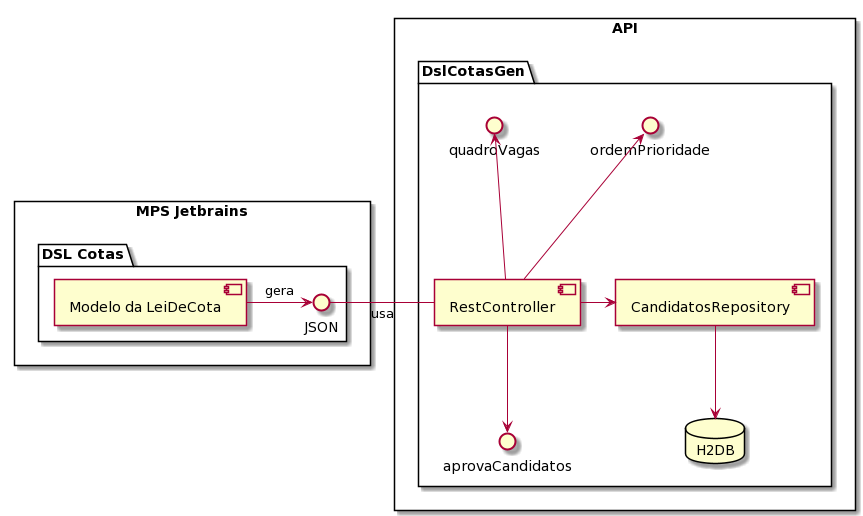
\includegraphics[width=0.88\textwidth]{chapters/dslcotas/api/imagens/apicomponentes.png}}

\par\medskip\textbf{Fonte:} Elaboração do autor (2020) \par\medskip

\end{figure}



\lstinputlisting[language=Java, 
caption=Endpoints no REST Controller  
,label=lst:restcontroller]{chapters/trechos_codigo/restcontroler.m}

\newpage
O método \texttt{quadro-vagas} (Código Fonte \ref{lst:restcontroller}, Linha 5), recebe como parâmetro a quantidade de vagas e o identificador da versão de lei, retornando uma lista de categorias com as respectivas siglas e quantidade de vagas (Figura \ref{fig:retquadrovagas}).

\begin{figure}[ht!]
\centering

\caption{\textmd{Retorno do método quadro-vagas}}
\label{fig:retquadrovagas}
\fcolorbox{gray}{white}{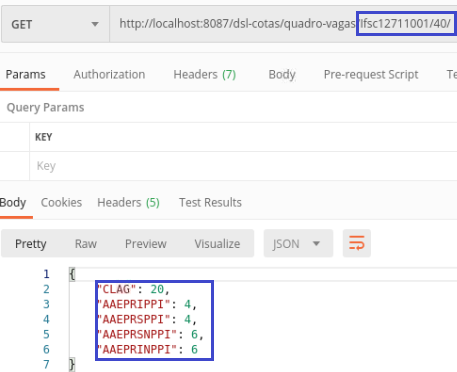
\includegraphics[width=0.98\textwidth]{chapters/dslcotas/api/imagens/retquadrovagas.png}}

\par\medskip\textbf{Fonte:} Elaboração do autor (2020) \par\medskip

\end{figure}



A aprovação é realizada no método \texttt{aprova-candidatos} (Código Fonte \ref{lst:restcontroller}, Linha 8), que recebe adicionalmente o parâmetro da lista de candidatos que deve ser processada. O seu retorno se dá por meio da mesma lista de candidatos, no entanto, já com a identificação da categoria de aprovação, conforme a versão da lei de cotas desejada (Figura \ref{fig:retaprovacandidatos}).
\begin{figure}[ht!]
\centering

\caption{\textmd{Retorno do método aprova-candidatos}}
\label{fig:retaprovacandidatos}
\fcolorbox{gray}{white}{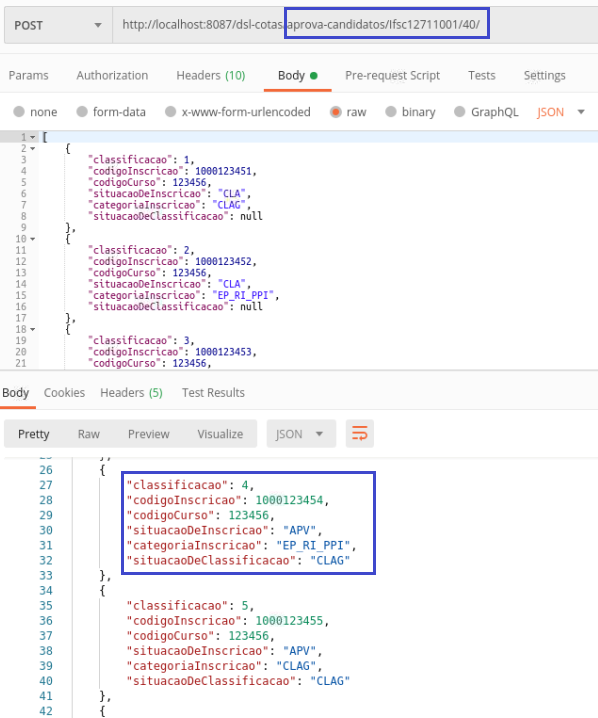
\includegraphics[width=0.88\textwidth]{chapters/dslcotas/api/imagens/retaprovacaocandidatos.png}}

\par\medskip\textbf{Fonte:} Elaborada pelo autor (2020). \par\medskip

\end{figure}


A lista de candidatos é composta pela ordem de classificação, o código de inscrição, o código do curso a que o candidato concorre, a situação de inscrição, categoria de concorrência selecionada na inscrição e a situação de classificação. O campo \texttt{situacaoDeInscricao} inicia com a situação classificado (CLA), para que após o processamento somente os candidatos aprovados sejam marcados como aprovados (APV). A categoria de classificação conforme o sistema de cotas é retornada no campo \texttt{situacaoDeClassificacao}.

\newpage
A interface de ordem de prioridade é atribuída ao método \texttt{ordem-prioridade} (Código Fonte \ref{lst:restcontroller}, Linha 13), esse possui apenas o parâmetro identificador da lei e devolve a lista de siglas conforme a definição de prioridade feita pelo usuário na DSL Cotas (Figura \ref{fig:retordemprioridade}).

\begin{figure}[ht!]
\centering

\caption{\textmd{Retorno do método ordem-prioridade}}
\label{fig:retordemprioridade}
\fcolorbox{gray}{white}{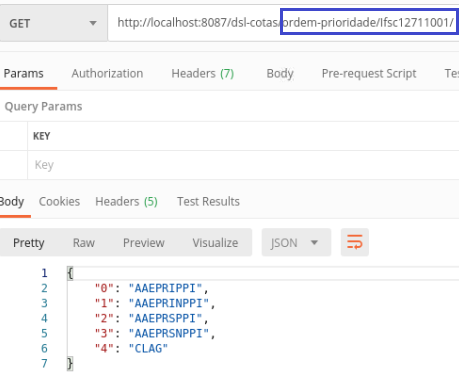
\includegraphics[width=0.88\textwidth]{chapters/dslcotas/api/imagens/retordemprioridade.png}}

\par\medskip\textbf{Fonte:} Elaborada pelo autor (2020). \par\medskip

\end{figure}


\newpage
No Capítulo seguinte serão apresentados os procedimentos metodológicos utilizados na pesquisa.